\section{Results}
\label{sec:results}

\subsection{Simulator credibility result}

The accepted Gate 3 record contains 67 evaluable checks and zero failures.
The result includes the Earth-only diagnostic chain that localized the original
J2 discrepancy to a coefficient-file delimiter problem rather than to the
integrator, time system, or initial state. Once the coefficient format was
repaired, the GMAT--Python comparison passed the unchanged position and
velocity thresholds across the eligible windows. The appropriate conclusion is
that the public simulator implements the tested scope consistently enough to
support the development benchmark. It is not a flight-readiness conclusion,
and RTC3 remains source-ineligible.

\subsection{Preregistered Gate 5 benchmark}

The Q01 quantum kernel did not satisfy the development trigger. Its mean NRMSE
was 0.646614, whereas C06 achieved 0.008739. The difference is sufficiently
large that it cannot be interpreted as a close race resolved by one
uncertainty statistic. No residual regime satisfied the frozen advance rule.
Gate 5 is therefore a valid technical FAIL for the Q01 model, task,
preprocessing, controls, and development population specified by the protocol.

Figure \ref{fig:gate5-curves} shows the pooled development evidence over the
authorized rungs and matched PCA dimensions. Configurations that did not
advance were stopped at their retention gate. Figure
\ref{fig:gate5-seeds} reports the selected-model distribution over the 20
frozen seed indices, and Fig. \ref{fig:gate5-trigger} places the trigger next
to its strongest classical and tuned dequantization controls. The three
figures should be read together: a model is not evaluated solely by a single
aggregate mean, but by its retained trajectory through the precommitted
decision rules.

\begin{figure}[t]
\centering

\includegraphics[width=\textwidth]{figures/gate5_development_learning_curves.png}
\caption{Gate 5 development learning curves and matched controls (RFIG-021).
The evidence covers every authorized rung and matched PCA dimension. This is
development model-selection evidence only.}
\label{fig:gate5-curves}
\end{figure}

\begin{figure}[t]
\centering

\includegraphics[width=0.92\textwidth]{figures/gate5_selected_model_seed_summary.png}
\caption{Twenty-seed summary of selected Gate 5 models (RFIG-022). Seed
variation is reported as a stability diagnostic, not as final-test evidence.}
\label{fig:gate5-seeds}
\end{figure}

\begin{figure}[t]
\centering
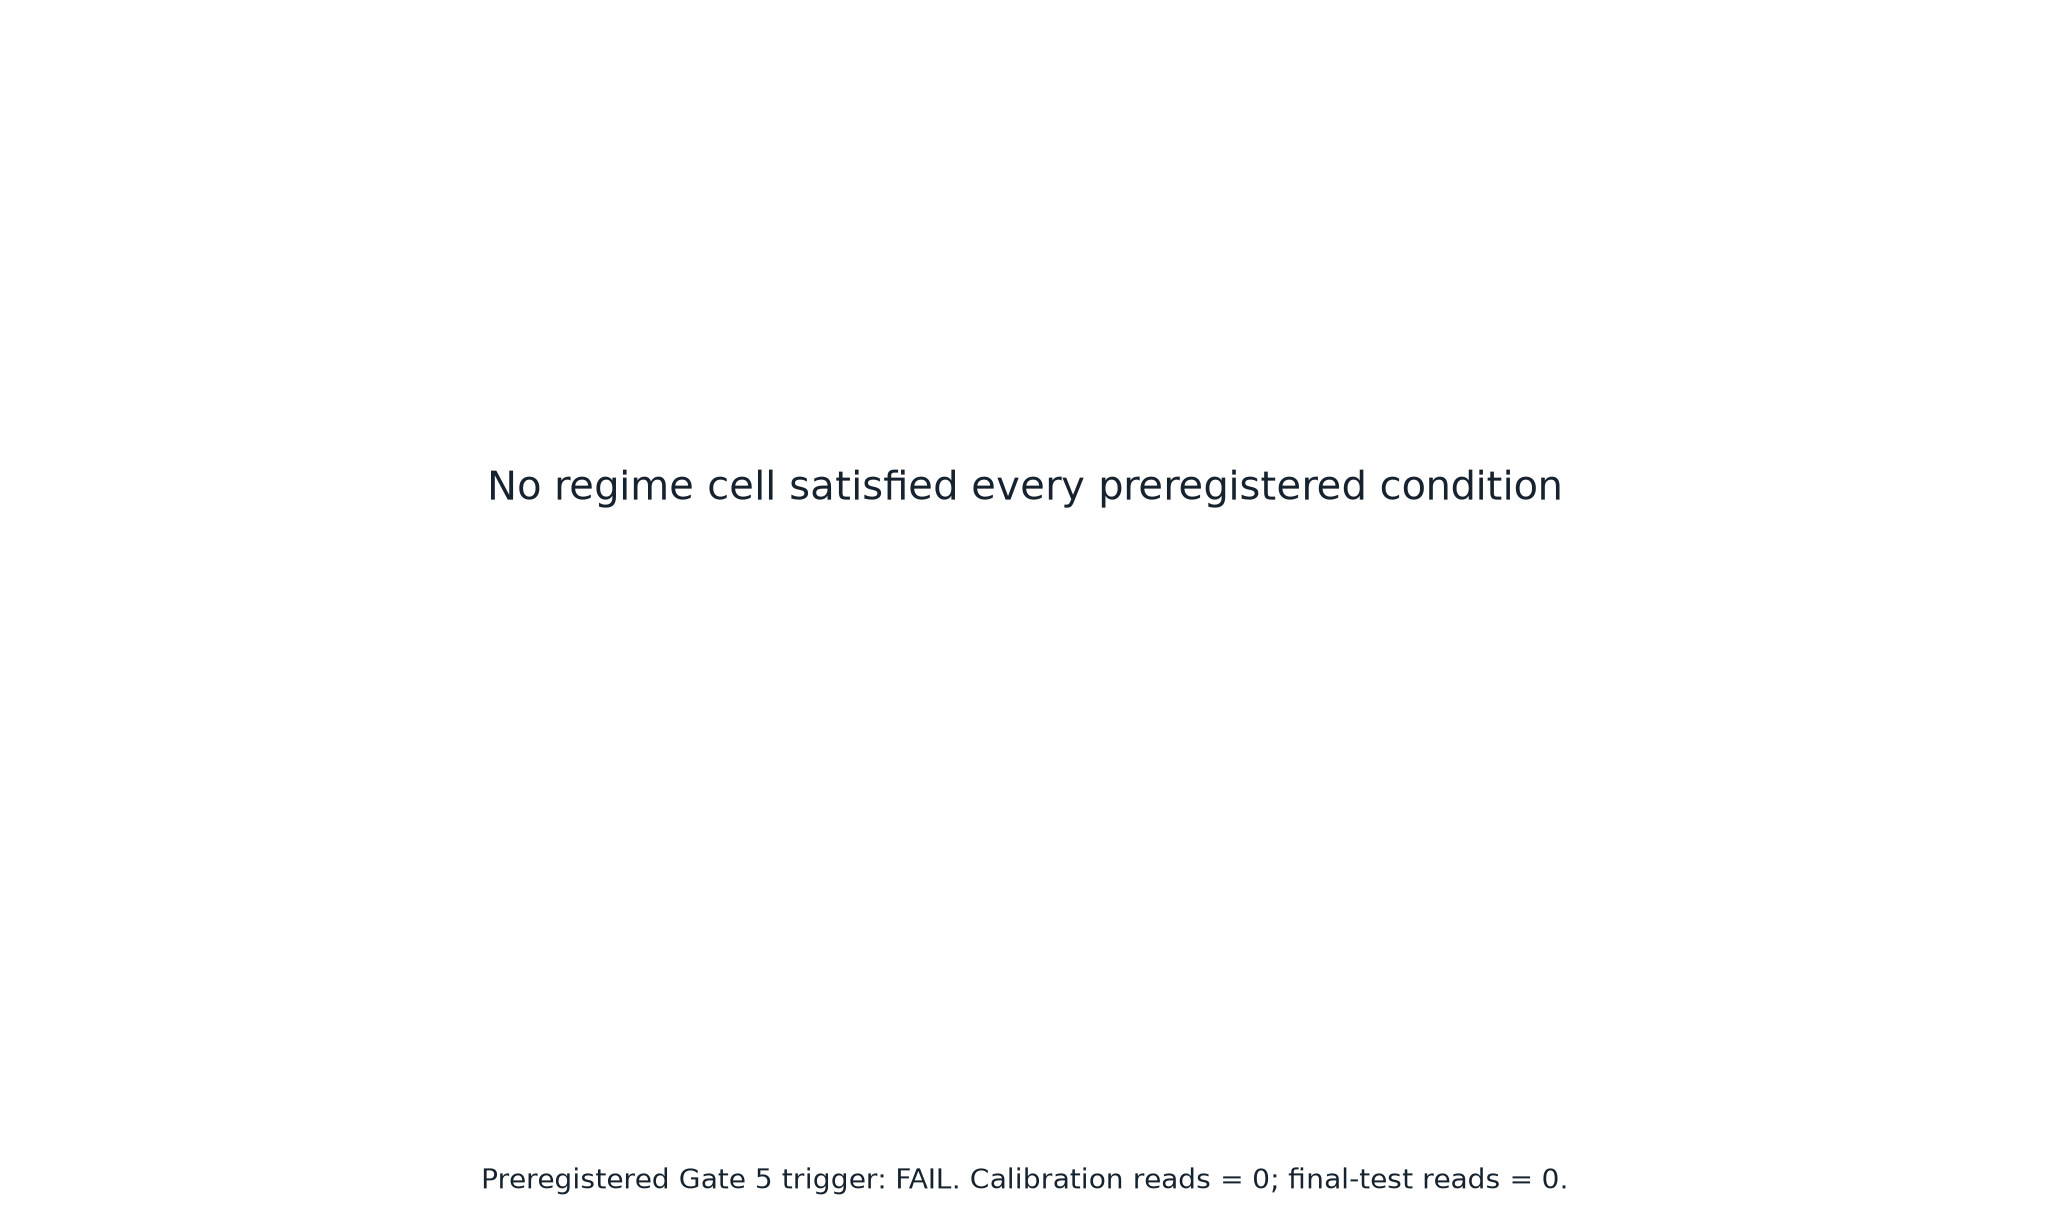
\includegraphics[width=0.92\textwidth]{figures/gate5_algorithm_trigger_regime_control.png}
\caption{Preregistered algorithm-trigger regime controls (RFIG-023). A
passing development trigger would have supported consideration of one further
algorithm study, not quantum advantage or operational deployment.}
\label{fig:gate5-trigger}
\end{figure}

Q02 and Q03 require a precise reading. They completed their authorized tasks,
but they did not satisfy the frozen eligibility condition for later rungs and
seed reruns. They are recorded as
\texttt{not\_reached\_under\_frozen\_eligibility}. Treating this state as a
failed experiment would overstate the evidence; treating it as an unreported
potential success would ignore the protocol. The paper reports the actual
decision state.

\begin{table}[t]
\caption{Primary and exploratory QML endpoints from the frozen evidence package. All values are development-only. Lower NRMSE and Brier score are better; higher recall is better for retaining actually feasible plans. The feasibility endpoint uses the fixed 0.5 threshold.}
\label{tab:gate5-results}
\centering
\footnotesize
\begin{tabularx}{\textwidth}{@{}>{\raggedright\arraybackslash}p{0.18\textwidth}>{\raggedright\arraybackslash}p{0.29\textwidth}Y@{}}
\toprule
Stage & Model and metric & Development result and meaning \\
\midrule
Primary Gate 5 & Fidelity quantum kernel (Q01); mean NRMSE & Q01: 0.646614; physics-residual C06: 0.008739. Protocol FAIL; no predefined subgroup passed. \\
Projected follow-up & Projected quantum kernel (Q01b; P001); mean NRMSE & Q01b: 0.661207; C06: 0.006833. Exploratory negative; about 97 times the C06 error. \\
Feasibility follow-up & Feasibility-only quantum kernel (FQK; P001); recall at 0.5 & Recall: 0.108860. It retained only 10.9\% of actually feasible cases, and classical controls were stronger. \\
Future lesson & Calibrated logistic model; feasible-case recall and Brier score & Recall: 0.804253; Brier: 0.142231. Protocol-design signal, not a safety result. \\
\bottomrule
\end{tabularx}
\end{table}


\subsection{Post-Gate 5 exploratory tracks}

Q01b tested whether changing the quantum readout while keeping the same
development discipline could materially alter the result. It did not. Q01b
attained mean NRMSE 0.661207, compared with 0.006833 for C06, a relative gap
of 95.77 times. Figure \ref{fig:q01b-curves} presents its learning curves
against the source-matched controls, while Fig. \ref{fig:q01b-geometry}
reports the projected-kernel geometry and dequantization diagnostics. These
are useful negative data: for this projected feature map, the representation
did not capture the residual structure better than the classical controls.
They do not establish that projected quantum kernels cannot work on any other
physical problem.

\begin{figure}[t]
\centering
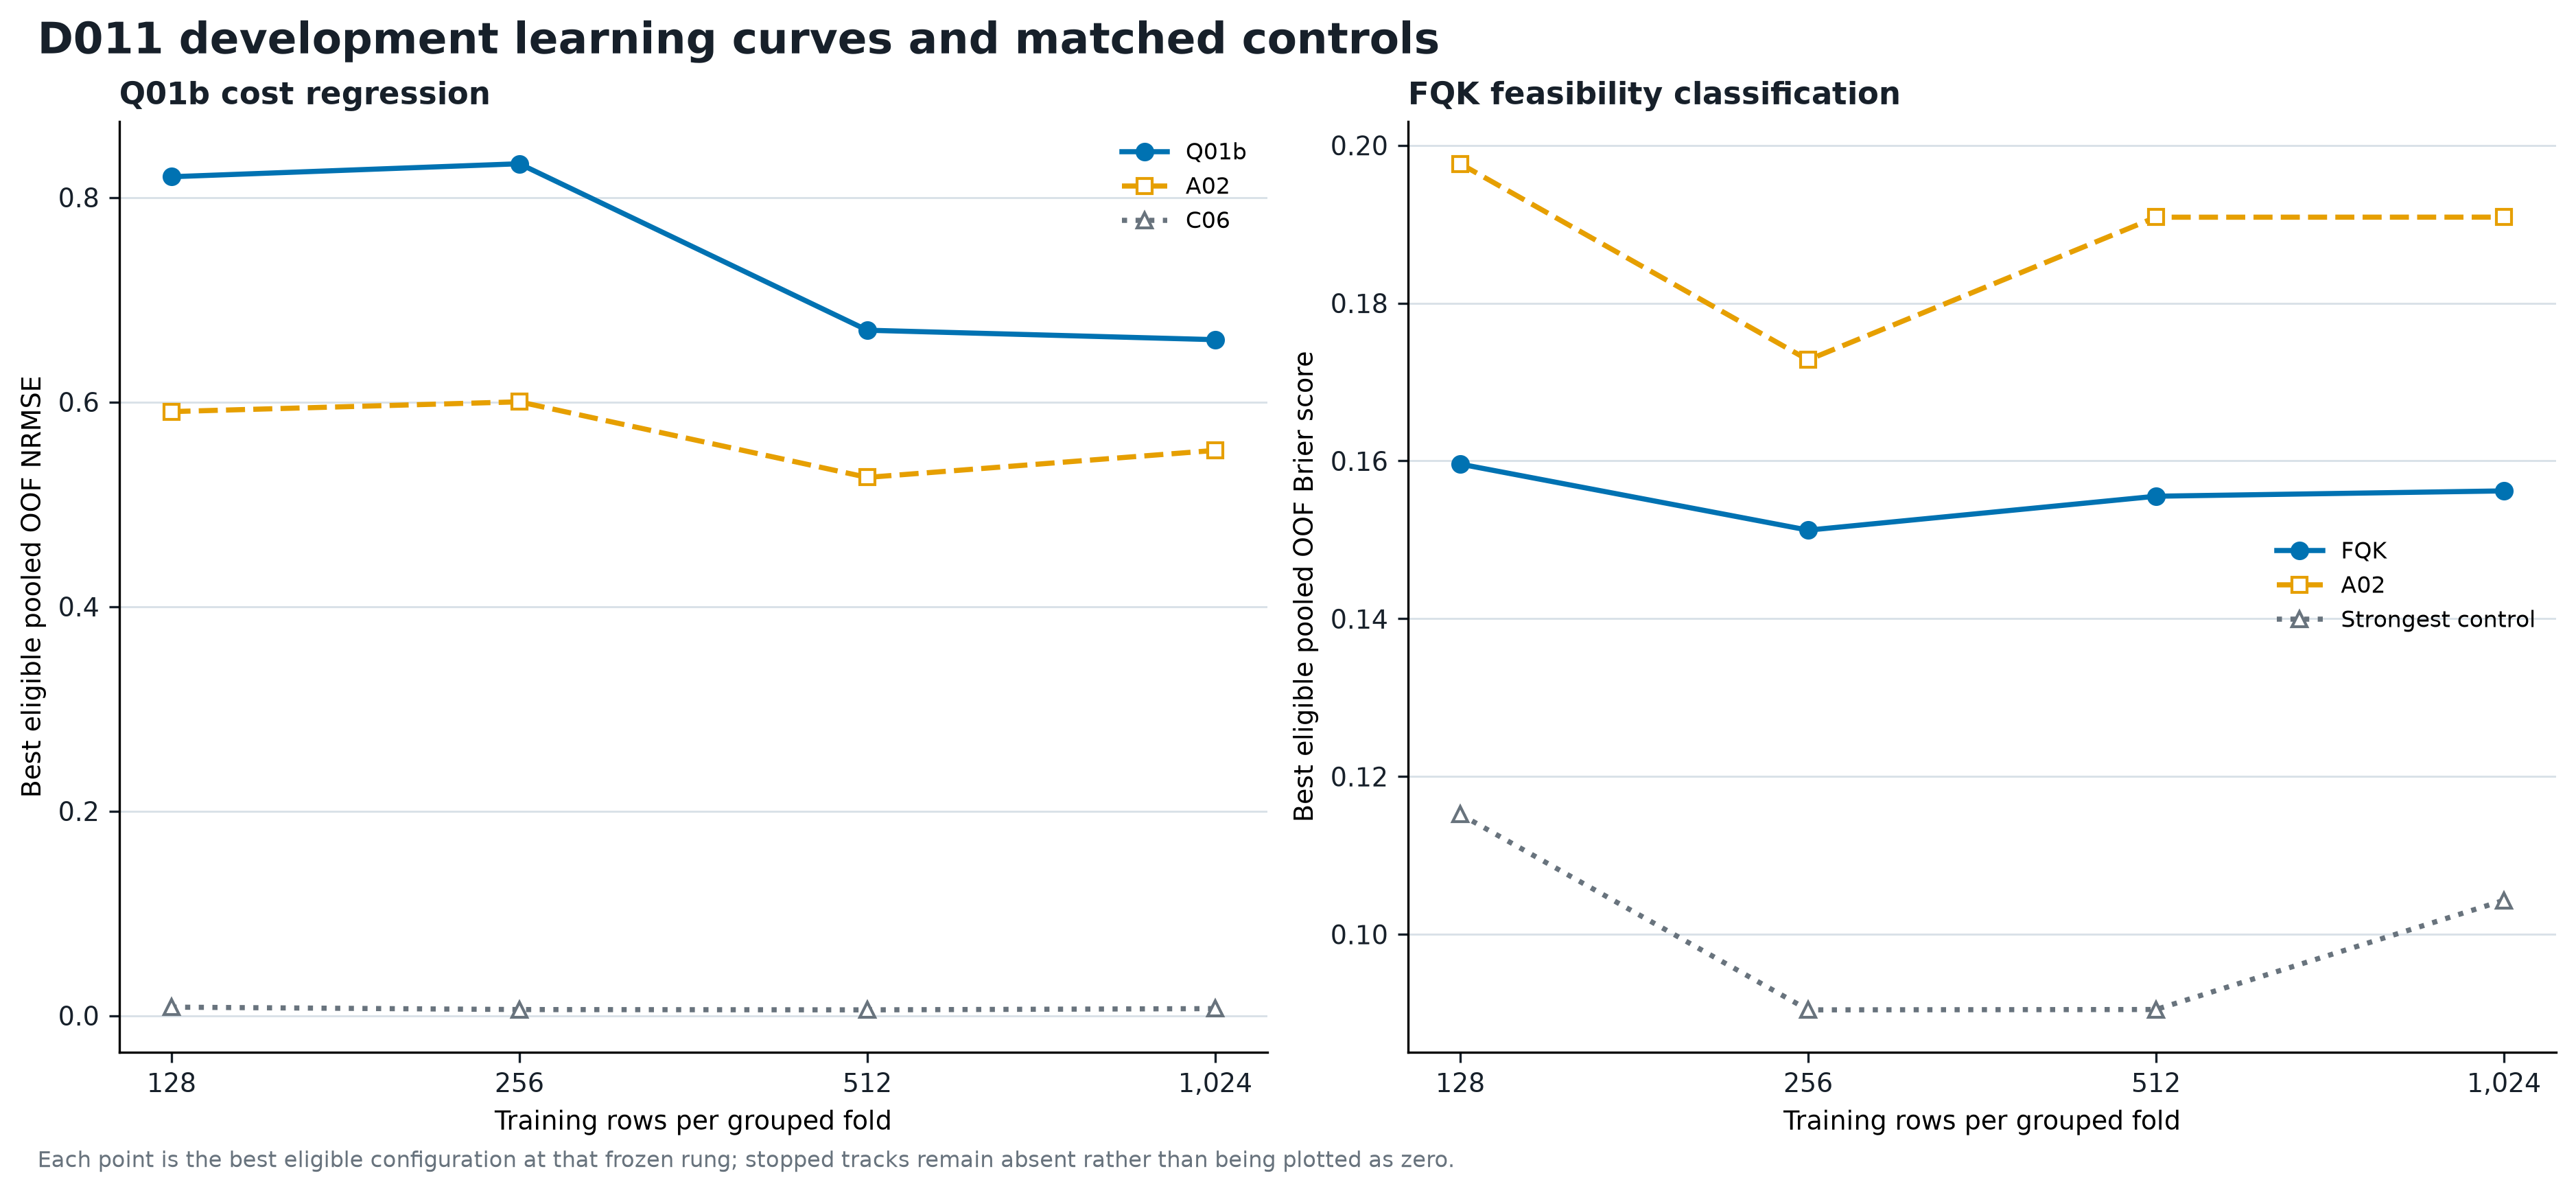
\includegraphics[width=\textwidth]{figures/post_gate5_d011_learning_curves.png}
\caption{D011/P001 projected-kernel learning curves and matched controls
(RFIG-026). The figure is development-only exploratory evidence and does not
revise the Gate 5 decision.}
\label{fig:q01b-curves}
\end{figure}

\begin{figure}[t]
\centering
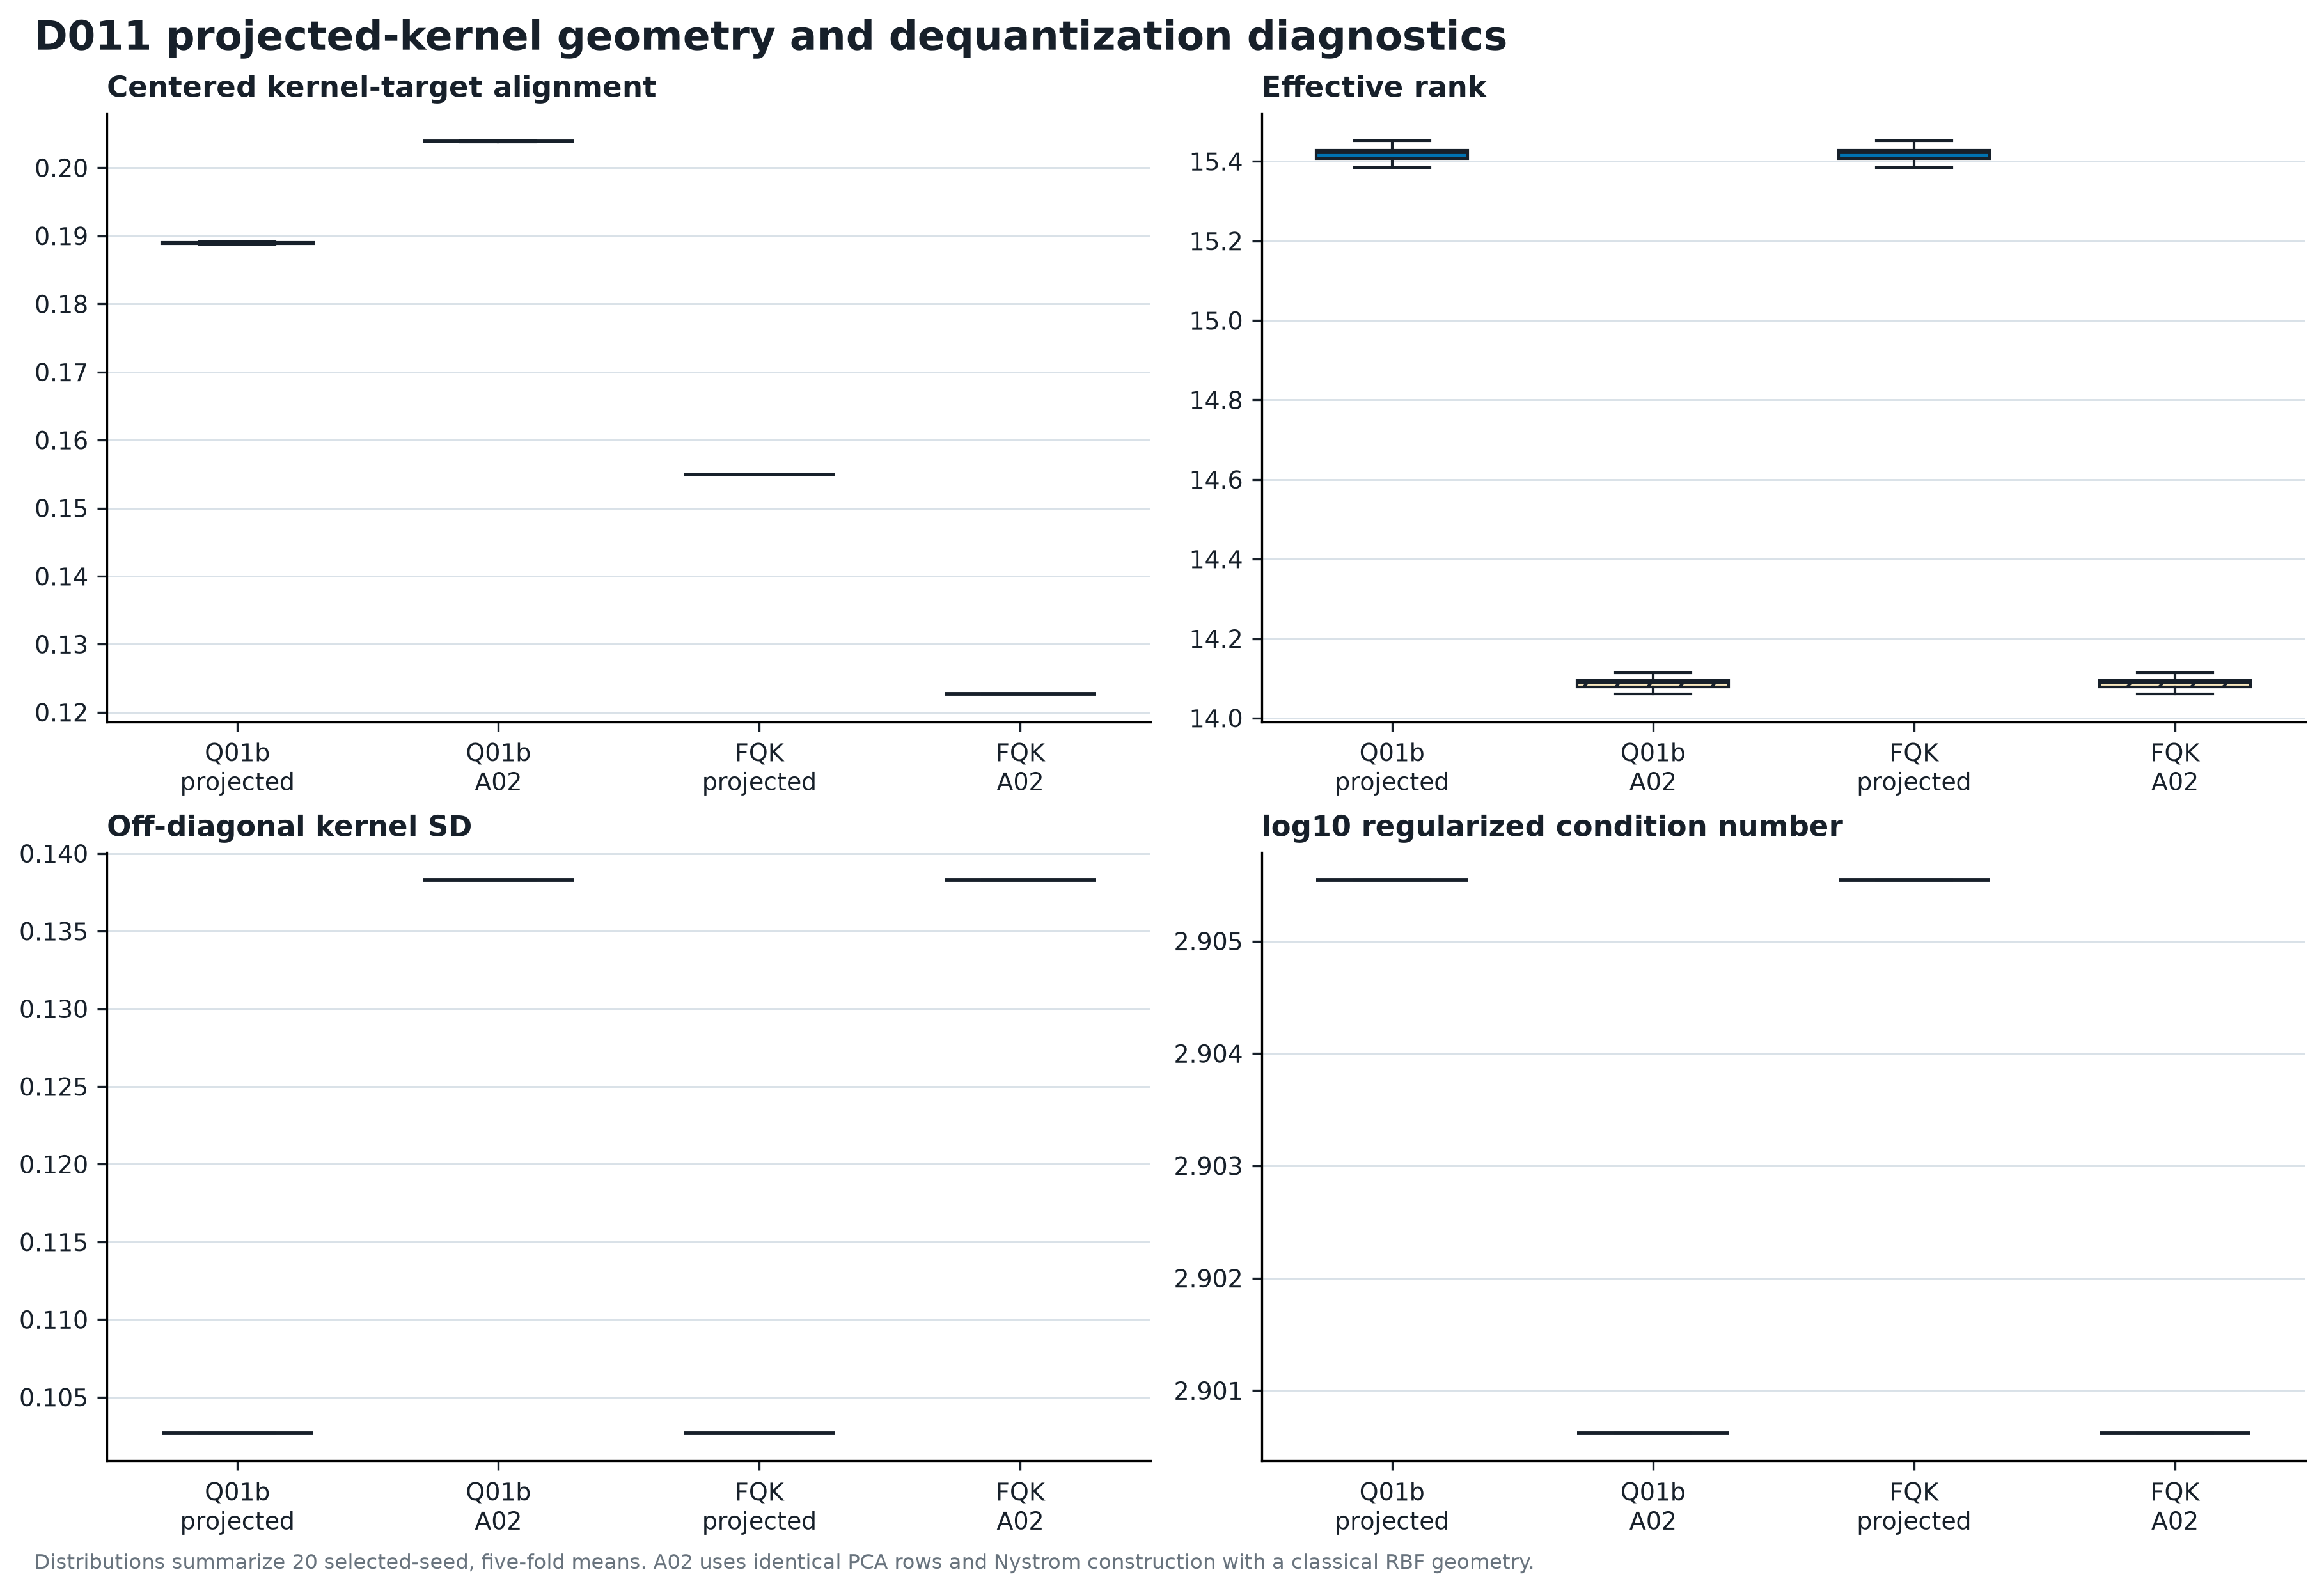
\includegraphics[width=\textwidth]{figures/post_gate5_d011_kernel_diagnostics.png}
\caption{Projected-kernel geometry and dequantization diagnostics (RFIG-027).
Selected projected kernels are compared with A02 classical RBF geometry on the
same fold-local PCA rows and Nystrom construction.}
\label{fig:q01b-geometry}
\end{figure}

The FQK classification track separates discrimination from a safety-filter
interpretation. It achieved AUROC 0.7436 and Brier score 0.1561, but recall at
the fixed threshold was only 0.1089. In a setting where missed unsafe cases
are material, the latter outcome prevents promotion to a safety-filter signal.
The endpoint plot in Fig. \ref{fig:fqk} makes this distinction visible. It is
not valid to call FQK useful for safety merely because one scalar metric is
above chance or because a quantum feature map was evaluated.

\begin{figure}[t]
\centering
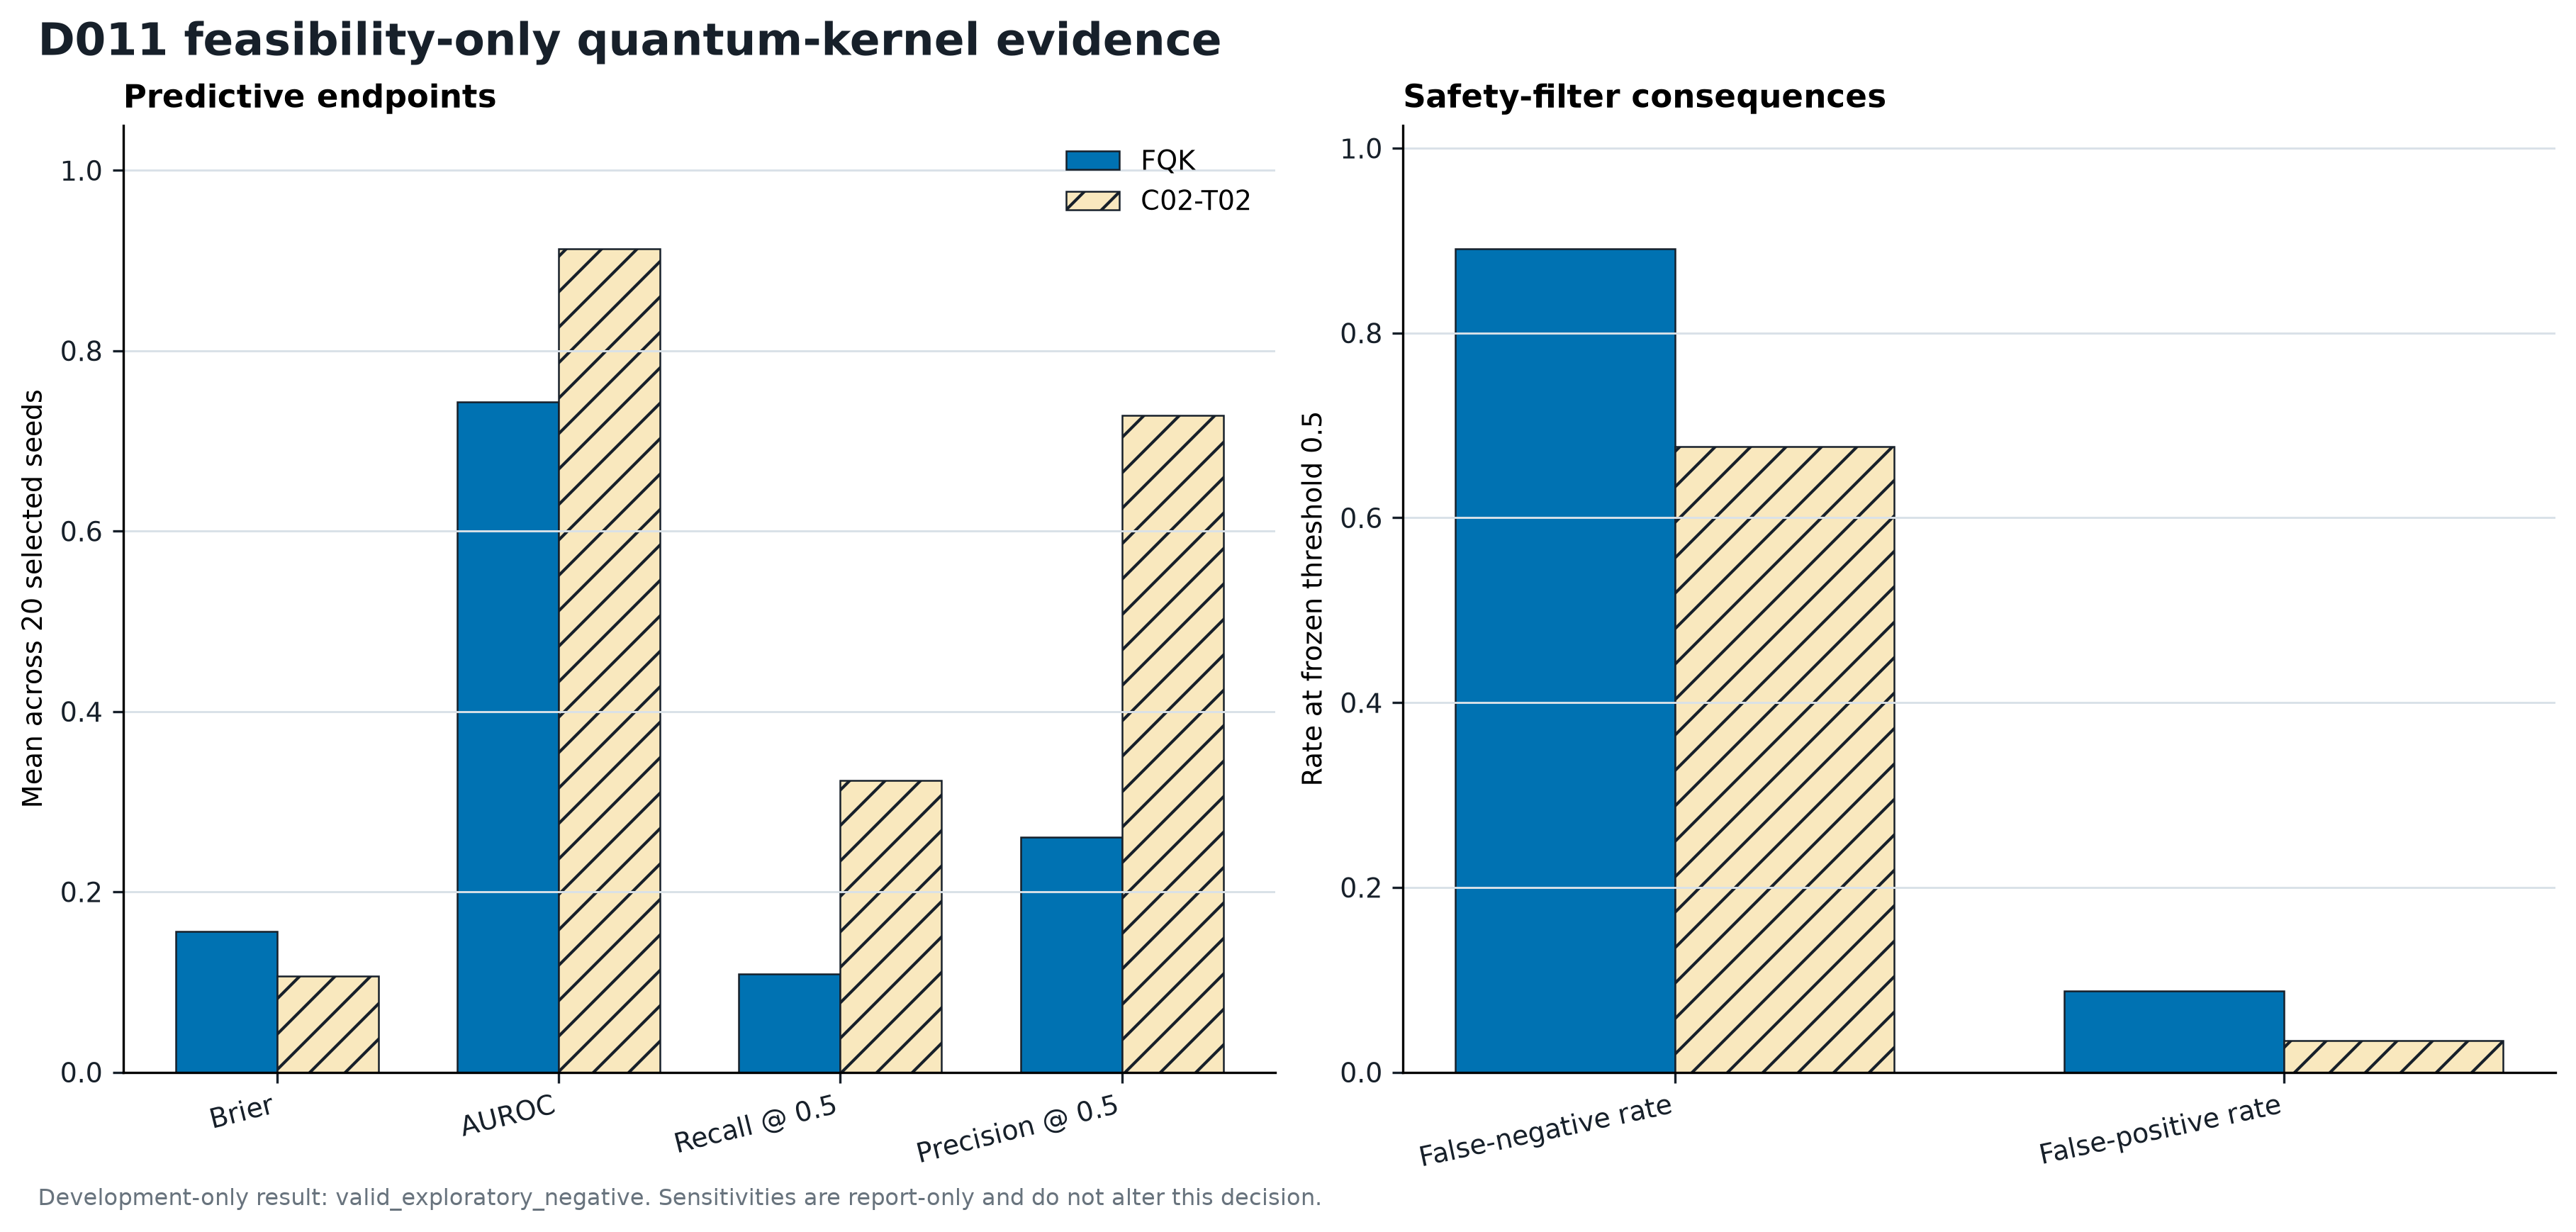
\includegraphics[width=\textwidth]{figures/post_gate5_d011_fqk_endpoints.png}
\caption{FQK predictive and safety-filter endpoints (RFIG-028). Brier,
discrimination, recall, precision, and consequence metrics are compared with
the strongest complete control. The frozen recall interpretation did not pass.}
\label{fig:fqk}
\end{figure}

The recall-first CSAFE-RF analysis provides a separate lesson for a future
protocol. A calibrated logistic model reached mean recall 0.804253 with
false-negative rate 0.195747 and Brier score 0.142231. That result identifies
an objective-design tension: a model selected only for calibration can miss an
unacceptable number of unsafe cases, whereas a future safety protocol should
prospectively define recall and calibration constraints together. CSAFE-RF was
not used to re-rank QML candidates, change a threshold, or authorize a mission
filter.

\subsection{Closed successor branch D034--D049}

The closed successor branch contains 16 prospectively bounded candidates. All
read the development scope only, used 39,000 development rows per campaign,
and completed with the recorded status
\texttt{complete\_valid\_negative}. The complete results are listed in Table
\ref{tab:successor-branch}. The table is intentionally included in full rather
than selecting only candidates with lower raw error than C06.

Several variants have a lower mean NRMSE than C06. This is a reason to inspect
the controls, not a reason to announce a quantum-specific result. The best raw
C06 comparison was D046, ORFRK-08-R2: NRMSE 0.0064363 versus 0.0068328 for
C06, an apparent 5.80\% reduction. Its matched second-stage RBF control,
TWO-RBF, attained 0.0067501. The candidate's improvement over that matched
classical alternative was therefore about 4.65\%, which is below the frozen
5\% branch-specific rule. The result does not meet the evidence standard for a
quantum-specific candidate.

\begin{figure}[t]
\centering
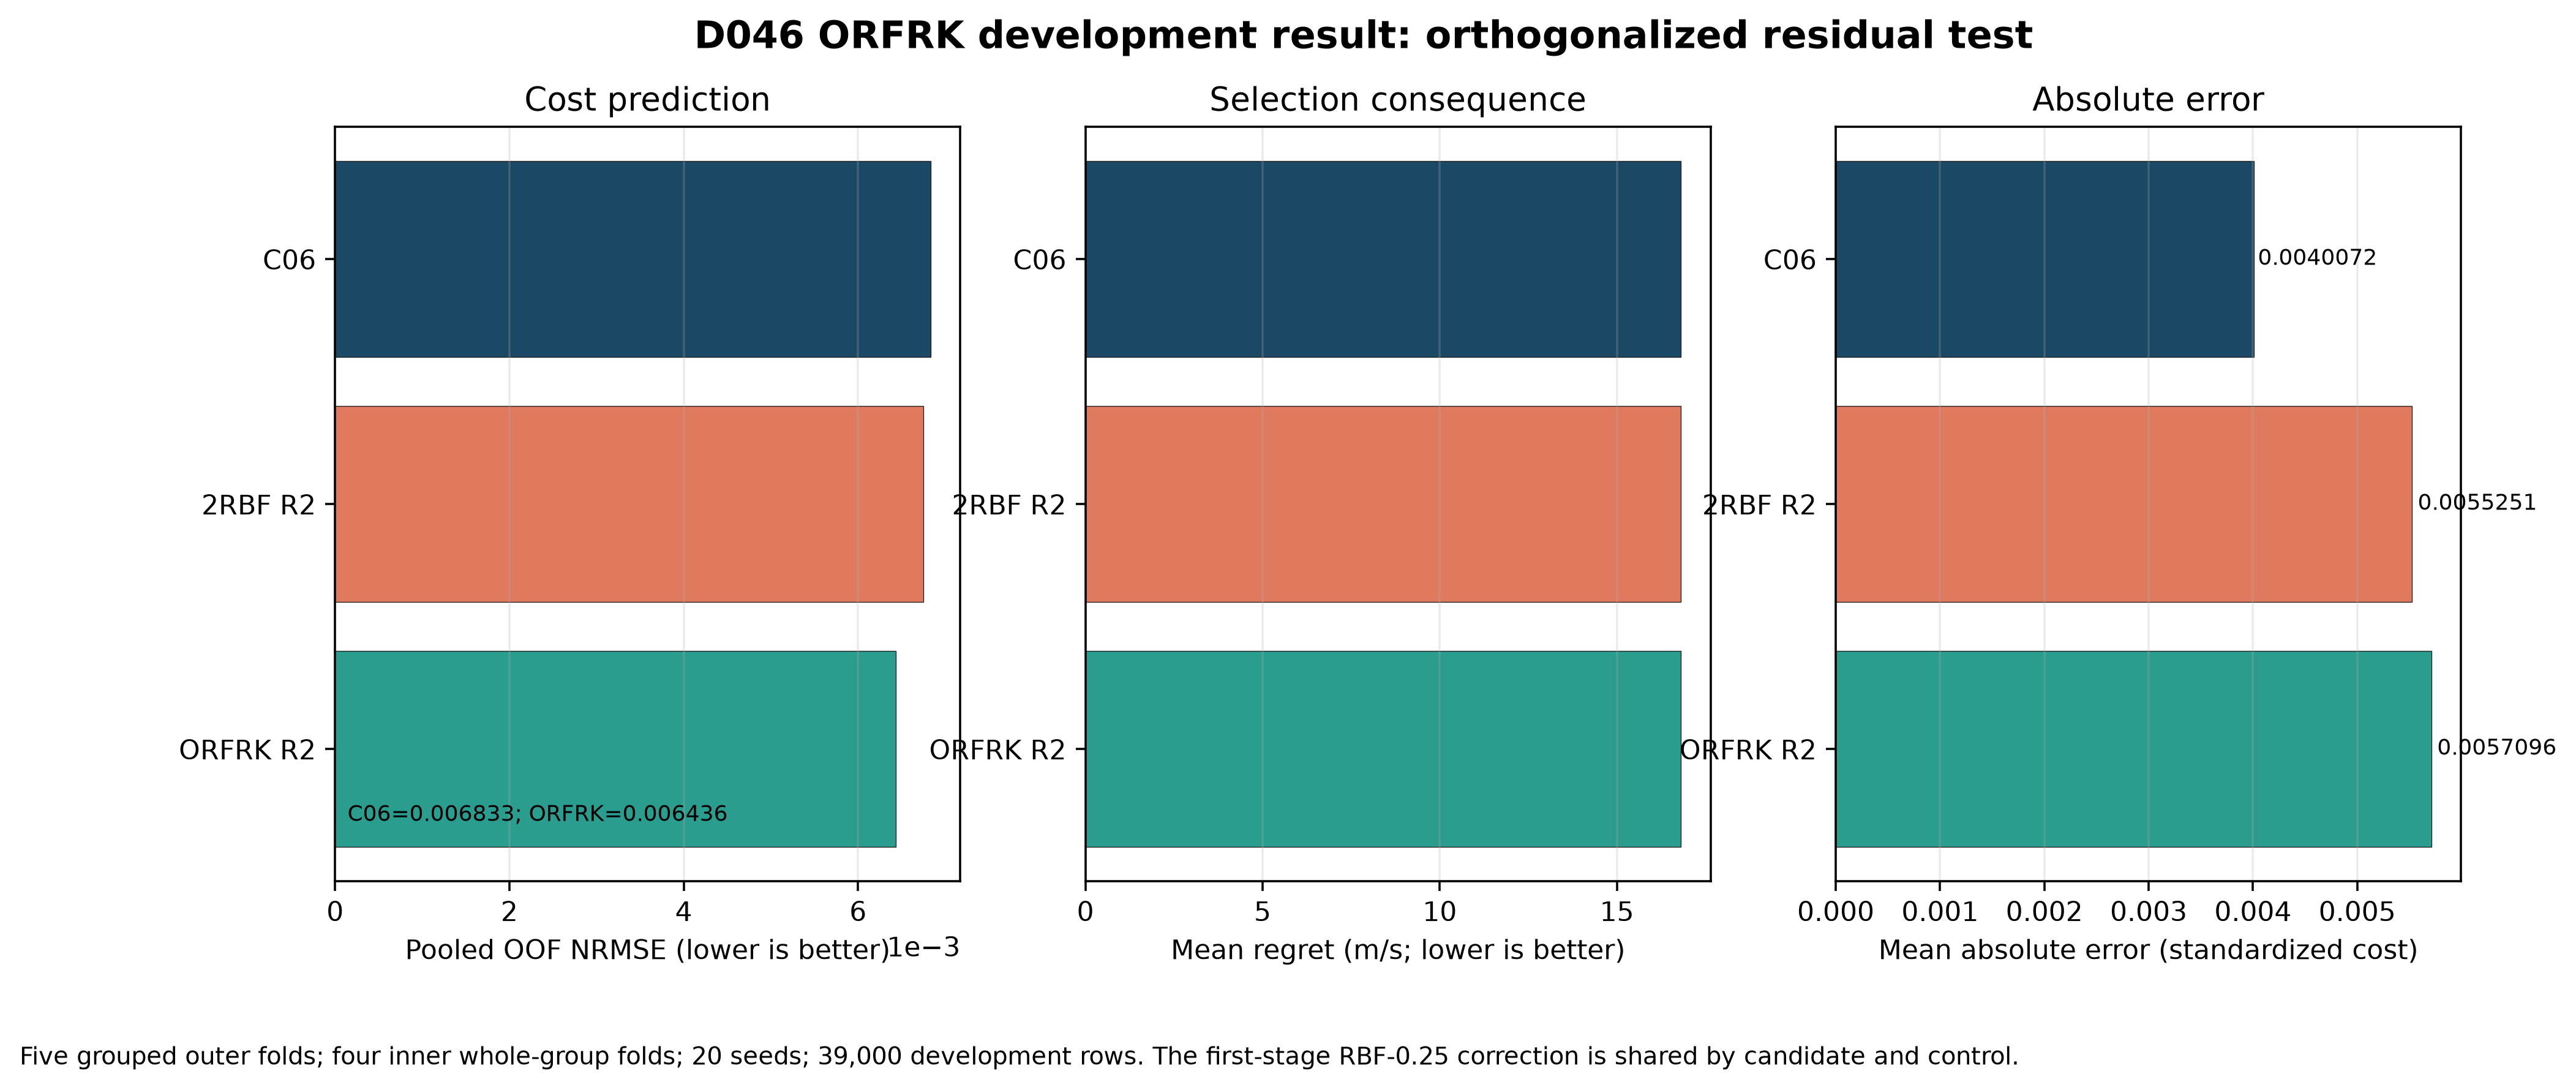
\includegraphics[width=\textwidth]{figures/post_gate5_d046_orfrk_result_comparison.png}
\caption{D046 ORFRK result comparison (RFIG-078). The q=8 candidate and a
matched second-stage RBF control are compared after a shared RBF-0.25
correction. Lower raw error than C06 is not sufficient for a QML claim.}
\label{fig:orfrk-result}
\end{figure}

\begin{figure}[t]
\centering
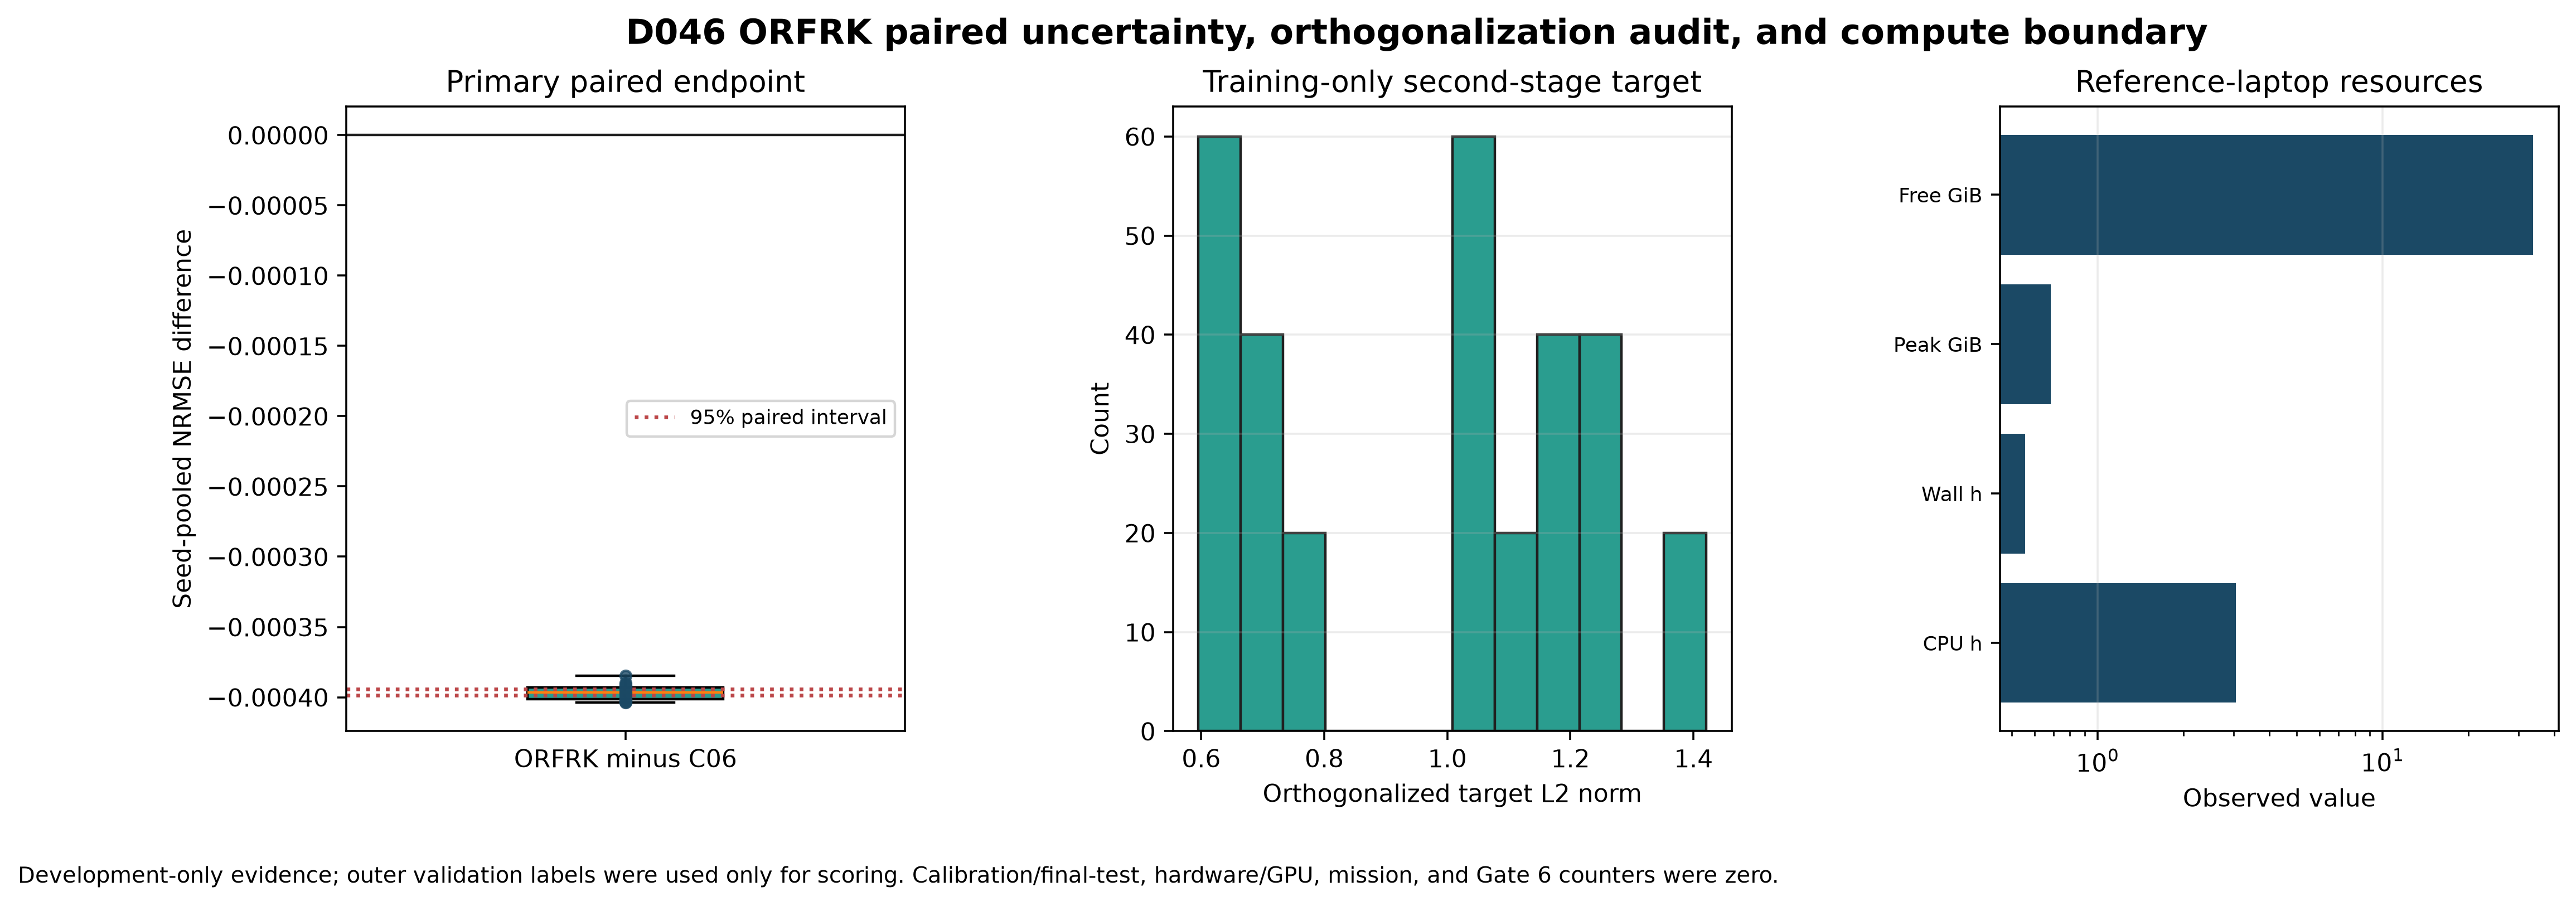
\includegraphics[width=\textwidth]{figures/post_gate5_d046_orfrk_audit_resources.png}
\caption{D046 paired audit and resource boundary (RFIG-079). The figure
reports the paired endpoint, training-only orthogonalization checks, integrity
evidence, and reference-laptop resources. It is not hardware or GPU evidence.}
\label{fig:orfrk-audit}
\end{figure}

\small
\begin{table}[!t]
\caption{Closed D034--D049 successor branch. Candidate names are immutable protocol IDs; their definitions are preserved in the repository. Every row is a valid development-only negative. The C06 NRMSE was 0.006833 throughout. Lower NRMSE is better, and a negative paired difference favors the candidate over C06, but each branch also had to pass its matched-control and stopping rules.}
\label{tab:successor-branch}
\centering
\scriptsize
\setlength{\tabcolsep}{2pt}
\renewcommand{\arraystretch}{0.92}
\begin{tabular}{@{}p{0.09\textwidth}p{0.24\textwidth}p{0.15\textwidth}p{0.17\textwidth}p{0.25\textwidth}@{}}
\toprule
Decision & Candidate & \shortstack[l]{Candidate\\NRMSE} & \shortstack[l]{Difference\\vs C06} & \shortstack[l]{95\% paired\\interval} \\
\midrule
D034 & PRQK-08-N & 0.029326 & 0.022493 & [0.022486, 0.022500] \\
D035 & CFQSR-08-N & 0.013463 & 0.006630 & [0.006627, 0.006632] \\
D036 & TAPQK-08 & 0.010382 & 0.003549 & [0.003547, 0.003551] \\
D037 & TSQR-08-L025 & 0.006848 & 0.000015 & [0.000015, 0.000015] \\
D038 & GFRK-08-L010 & 0.006647 & -0.000186 & [-0.000187, -0.000184] \\
D039 & EC-GFRK-08-L010 & 0.006466 & -0.000366 & [-0.000368, -0.000365] \\
D040 & CE-GFRK-08-L010 & 0.006504 & -0.000329 & [-0.000330, -0.000328] \\
D041 & HEFRK-08-E050 & 0.006592 & -0.000241 & [-0.000242, -0.000240] \\
D042 & AGEFRK-08-ADAPT & 0.006524 & -0.000309 & [-0.000310, -0.000308] \\
D043 & SFRK-08-CV & 0.006445 & -0.000387 & [-0.000389, -0.000386] \\
D044 & NIFRK-08-NL & 0.006751 & -0.000081 & [-0.000084, -0.000079] \\
D045 & MSFRK-ALL & 0.006731 & -0.000102 & [-0.000103, -0.000100] \\
D046 & ORFRK-08-R2 & 0.006436 & -0.000397 & [-0.000399, -0.000394] \\
D047 & OMFRK-ALL & 0.006952 & 0.000119 & [0.000113, 0.000125] \\
D048 & NSORFRK-08 & 0.006590 & -0.000243 & [-0.000244, -0.000242] \\
D049 & SSORFRK-08 & 0.006566 & -0.000266 & [-0.000268, -0.000265] \\
\bottomrule
\end{tabular}
\renewcommand{\arraystretch}{1}
\end{table}

\normalsize

\subsection{Evidence accounting and closure}

Evidence accounting confirms that the reported conclusion follows the
authorized boundary. D006 completed 871 of 871 tasks, with zero task failures
and zero reads of calibration or final-test data. The D011-R1 exploratory
campaign read 39,000 development rows and zero locked rows. No hardware
quantum job, mission-loop run, Gate 6 run, or final-test evaluation occurred.

Figure \ref{fig:closure} summarizes the closure recommendation. It reports
that no candidate is eligible for Gate 6; it does not represent an unexecuted
Gate 6 experiment. The experimental program was subsequently closed under
D055-C to permit publication preparation without turning future protocol ideas
into unapproved computation.

\begin{figure}[t]
\centering
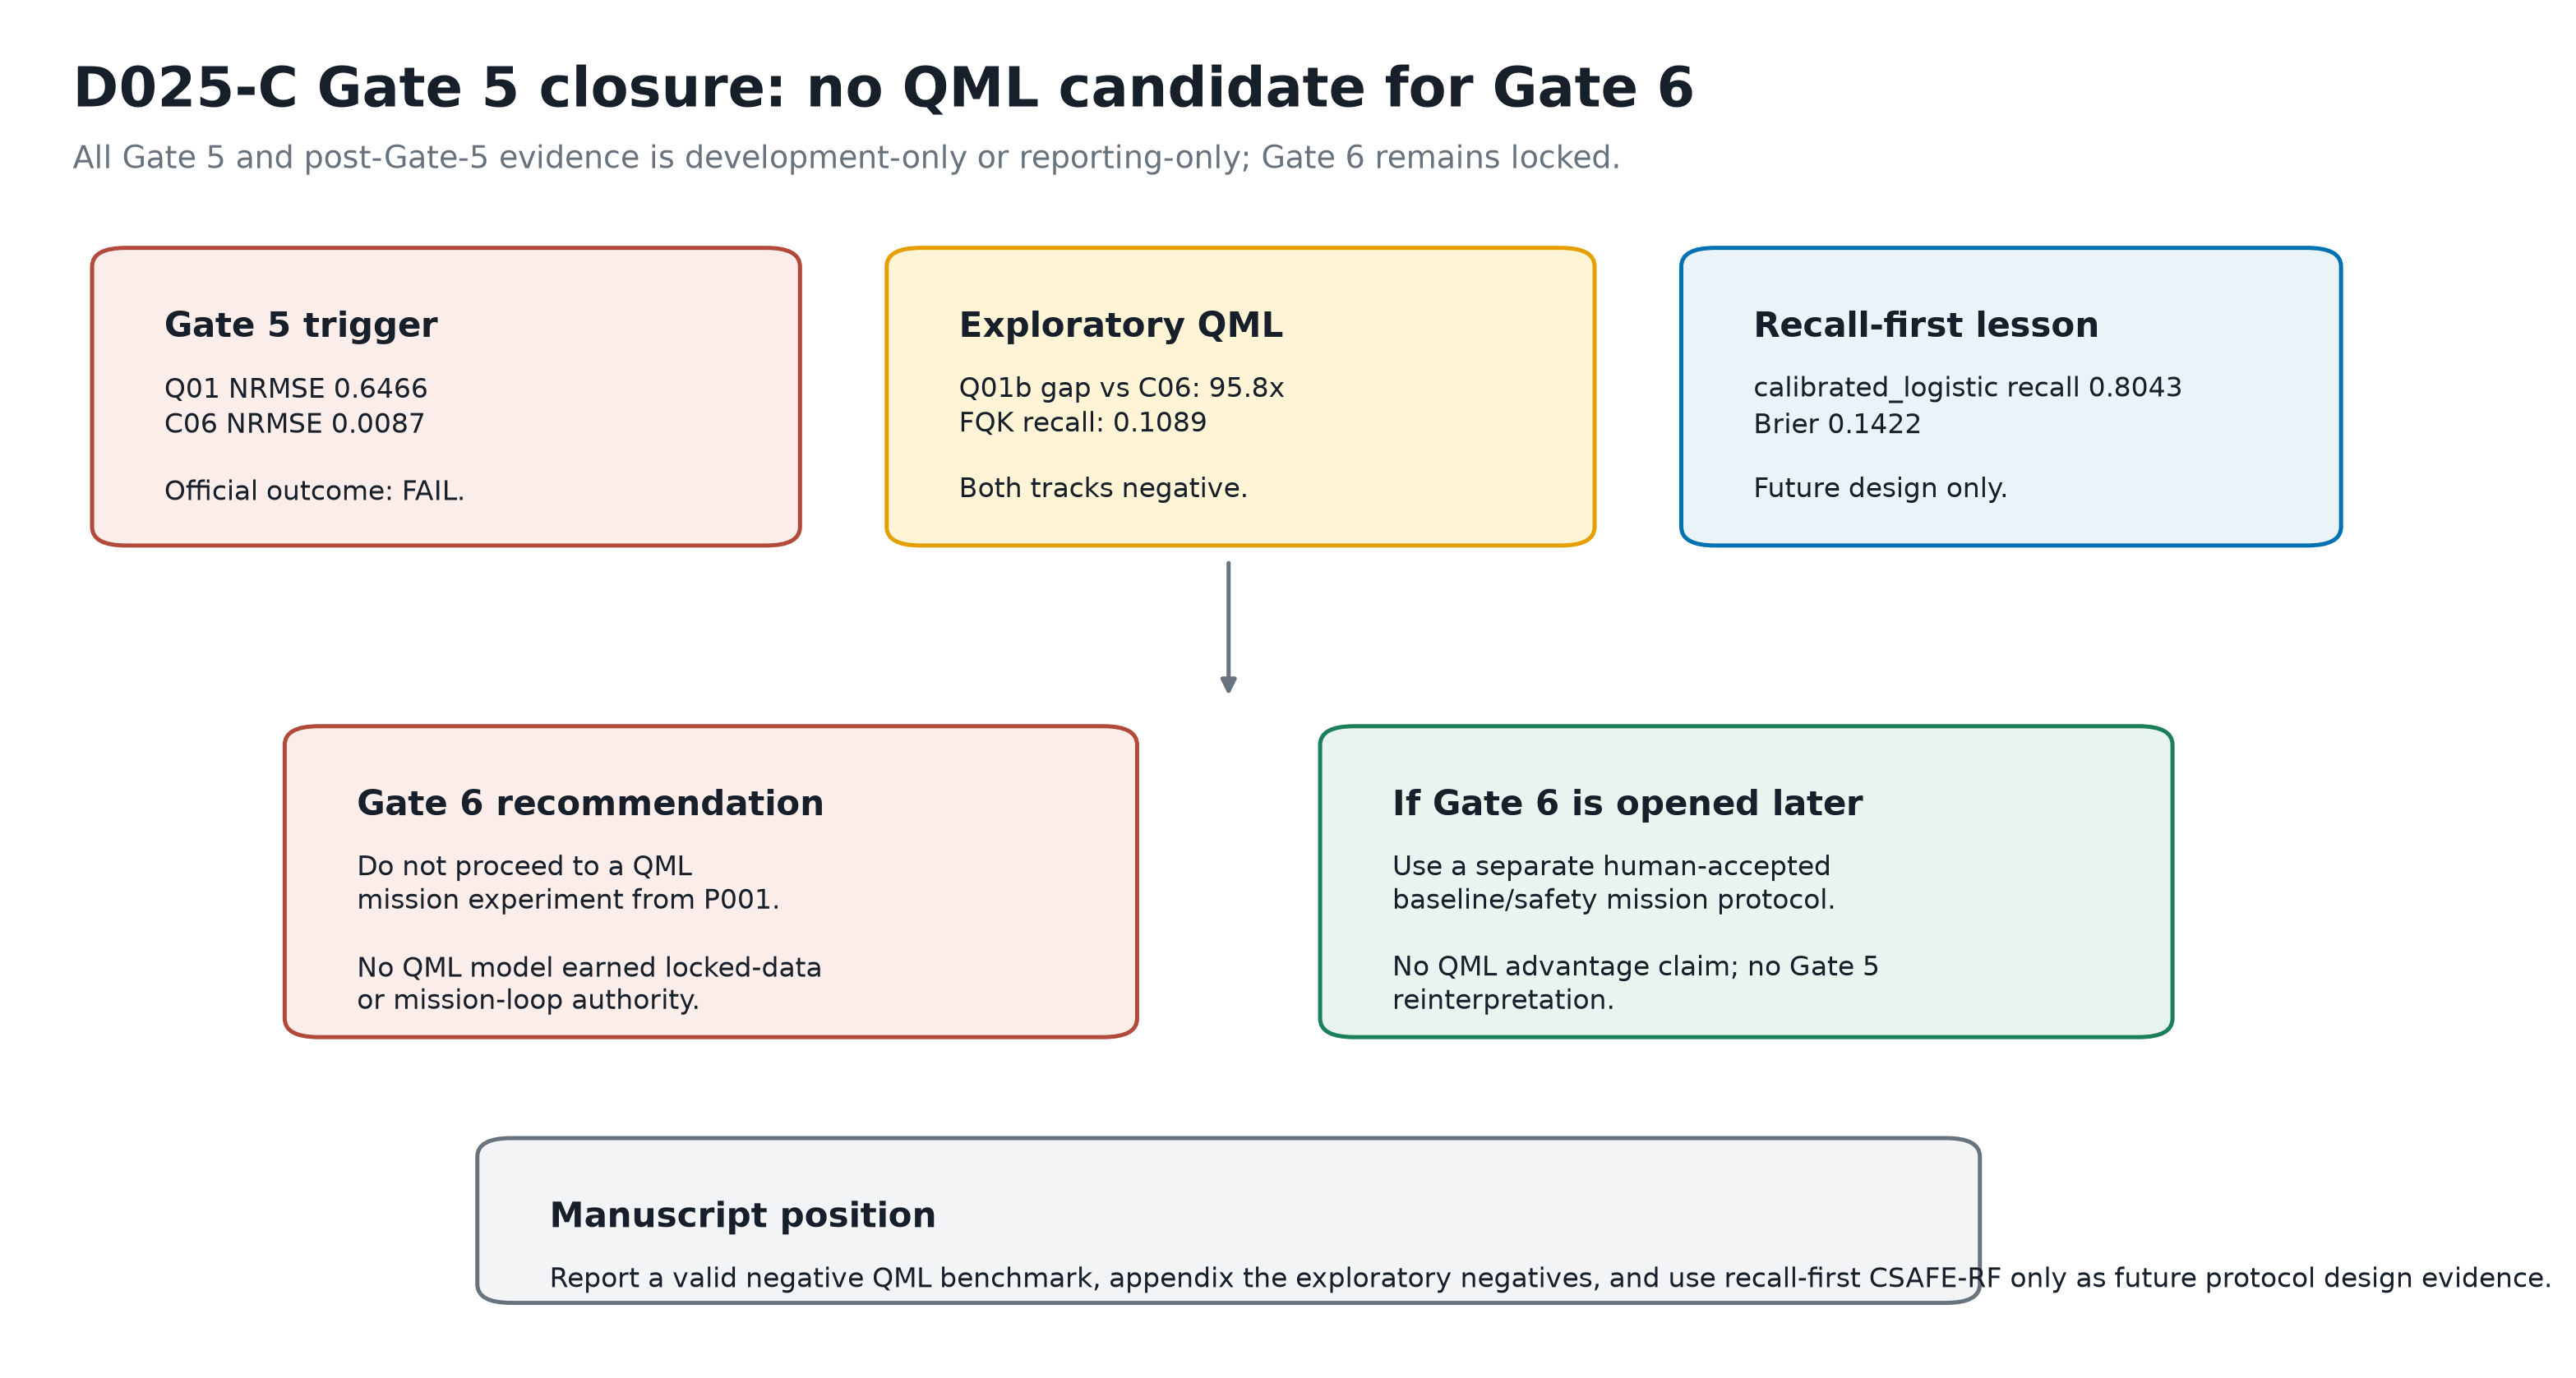
\includegraphics[width=\textwidth]{figures/post_gate5_d025_gate6_recommendation.png}
\caption{Gate 5 closure and Gate 6 recommendation (RFIG-044). No QML candidate
from the closed evidence branches is eligible for Gate 6. This is a closure
recommendation, not a Gate 6 result.}
\label{fig:closure}
\end{figure}
